MDT's form the majority of the precision-tracking chambers used in the MS, covering up to $|\eta| < 2.7$, except in the innermost end-cap layer where coverage is limited to $|\eta| < 2.0$. There are approximately 1,100 MDT chambers through the entire ATLAS detector, and approximately 350,000 drift tubes. Each chamber consists of one or two multilayers, with each multilayer consisting of 3 to 4 layers of drift tubes, and each layer containing 30 to 100 tubes.

In the barrel region, MDT's are located on and between the eight coils of the barrel toroid magnets. They are arranged in three concentric cylindrical layers around the $z$-axis with inner radii of approximately 5 m, 7.5 m and 10 m. MDT chamber size increases with radial distance from the IP to maintain angular resolution\@.

In the end-cap region, MDT's are placed behind the end-cap toroid magnets. The MDT's are arranged in two large wheels located along the $z$-axis at distances of 14 m and 21.5 m. These wheels are placed perpendicular to the $z$-axis and extend radially outward.

MDT's rely on drift tubes to measure the position of charge particles. In the MS, the drift tubes are approximately 30 mm in diameter and operate with a combination of Argon (93\%) and Carbon Dioxide (7\%). As a muon passes through the tube, the gas ionizes releasing electrons that drift towards the central tungsten-rhenium wire which is kept at a 3080 V. 

A cross section view of the MDT system in the $r-z$ plane can be seen in Figure~\ref{fig:atlas_mdt_cross_section} and a diagram of an MDT chamber can be seen in Figure~\ref{fig:mdt_chamber}.

\begin{figure}[htp]
    \centering
    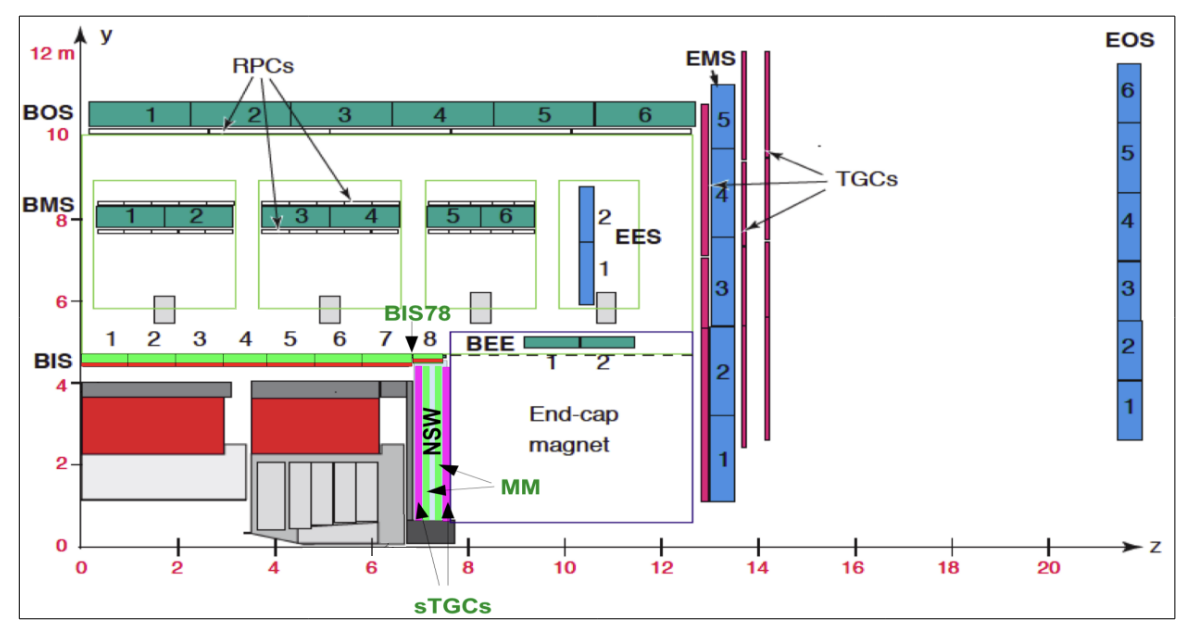
\includegraphics[width=0.8\textwidth]{figures/atlas/atlas_ms_run3_layout.png}
    \caption{Cross-section of the MDT system in the $r-z$ plane. The MDT's are located between the barrel toroid coils and the end-cap toroid coils. The MDT's are arranged in three cylindrical layers in the barrel region, and two large wheels in the end-cap region. The increasing size of the MDT's as distance from the IP increases is also seen. Taken from~\cite{atlas_mdt_cross_section}.}\label{fig:atlas_mdt_cross_section}
\end{figure}

\begin{figure}[htp]
    \centering
    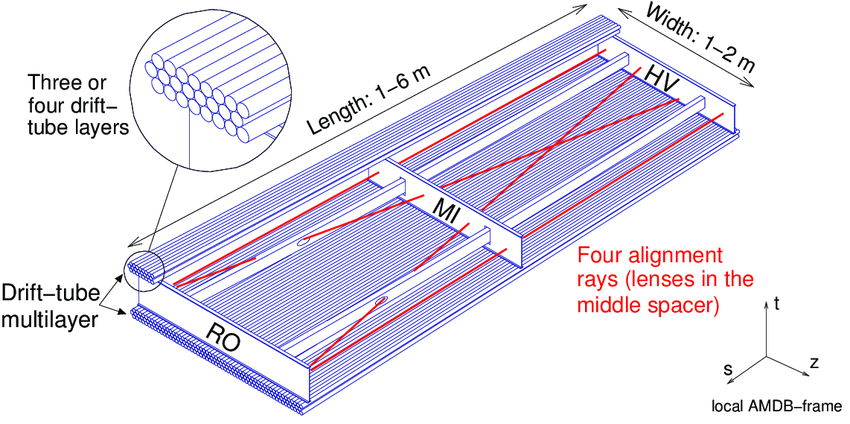
\includegraphics[width=0.8\textwidth]{figures/atlas/atlas_mdt_drifttube.png}
    \caption{Layout of a barrel MDT chamber. Drift tubes are arranged into two multilayers that are separated by a spacer. Each multilayer contains 3 or 4 layers of drift tubes. End-cap MDT chambers are trapezoidal in shape. Taken from~\cite{atlas_collaboration_paper}.}\label{fig:mdt_chamber}
\end{figure}